\documentclass{standalone}
\begin{document}
\markboth{SEGMENTATION MODELS COMPARISON}{APPENDIX}
\chapter*{Appendix - Segmentation Models Comparison}\addcontentsline{toc}{chapter}{Appendix - Segmentation Models Comparison}

MRI colorectal cancer segmentation is a particularly hard task to perform.
Among the issues, there is the quality of data (i.e. the presence of different tumor subtypes such as \textit{mucinous}), the medical annotations (subjected to operator expertise), the loss functions, and even model parameters that can affect the results of segmentation.\\
The aim of this Appendix is to give a comparison of two different CNN models, trained on the same data and medical annotations, changing the loss function and the number of epochs.
In particular, one consists of the model used in the implemented pipeline, Model 1, and the other one, Model 2, of the same architecture, that is U-net with EfficientNetb0 as a backbone, and the Dice binary cross-entropy (DCE) as Loss function.
The results and the specifications are reported in Table \ref{tab:comparison}.
\\
As you can see, by changing the Loss function and the number of epochs you can get a different performance as shown by the Dice Similarity Coefficient (DSC) score and the Loss one.
Model 1 got a DSC score that is higher than the one obtained by Model 2, meaning a better performance.
This is reflected even looking at the Loss score (lower the Loss score higher the performance).
\\
In Figure \ref{training1} and \ref{training2}, the curves of the training (blue) and validation (green) process for both the models are shown.
As you can see, Model 1 results more stable than Model 2 since the fluctuations of the DSC and the loss are more restrained.
\\
The difference in performances can also be appreciated by comparing the segmentation results with the ground-truth images.
This is shown in Figure \ref{predcomparison} and \ref{predcomparison2}.
The prediction is plotted as a probability density map between 0. and 1. as shown by the sequential colormap.
\\
You can notice that the results obtained from Model 1 are better than the ones obtained from Model 2.
In particular, Model 1 allows one to get better contours so as to be closer to the ground-truth image.
However, it must be said that Model 1 was trained for 150 epochs versus 100 epochs for Model 2.
Therefore, Model 1 has the benefit of more learning processes.
\\
The difference in performances can be better perceived in Figure \ref{predcomparisonoverlap} and \ref{predcomparisonoverlap2} where the ground-truth image and the predicted ones overlap the input image so embedding spatial information about patient's anatomy.
The prediction is plotted as a probability density map between 0. and 1. as shown by the sequential colormap.
\\
Even in this case, you can see how Model 1 segmentation results are more accurate than the ones obtained by Model 2.
As a matter of fact, Model 2 is able to correctly discriminate the tumor region but the contours are not very close to the ground truth ones like instead are for the predictions of Model 1.
In Figure \ref{predcomparisonoverlap2}, on second row, I also included a case of \textit{mucinous} tumor subtype.
This kind of tumor is characterized by bright tumoral areas on MRI scans, different from the \textit{adenocarcinomas} characterized by dark tumoral areas so the model can have more difficult in segmentation tasks.
Indeed, Model 2 correctly discriminate the tumor region but the contours are not very accurate like the ones obtained by Model 1 predictions.
\\
In the end, Model 1 has been proved to get better results compared to Model 2.
This was achieved only by using a different Loss function and rising the number of epochs while keeping the same model architecture, U-Net with EfficientNetb0 as a backbone.

\vfill

\begin{table}[htp]
	\centering
	\begin{tabular}{lccccc}
		\toprule
		  & \textbf{Architecture} & \textbf{Loss Function} & \textbf{Epochs} & \textbf{DSC} & \textbf{Loss} \\
	    \midrule
		Model 1  & U-Net, backbone & Dice Loss +   &  150 &  0.71 & 0.25\\
                & EfficientNetb0 &    Focal Loss              &      &   &   \\
         \midrule
		Model 2  & U-Net, backbone  & Dice binary  & 100 &  0.68 & 0.35 \\
        & EfficientNetb0 &   cross-entropy Loss               &      &   &   \\

		\bottomrule
	\end{tabular}
	\caption{Table of comparison between the two models. As you can see, by changing the loss function and the number of epochs you can get different performances.}
	\label{tab:comparison}
\end{table}

\vfill


\begin{figure}[htp]
    \centering
    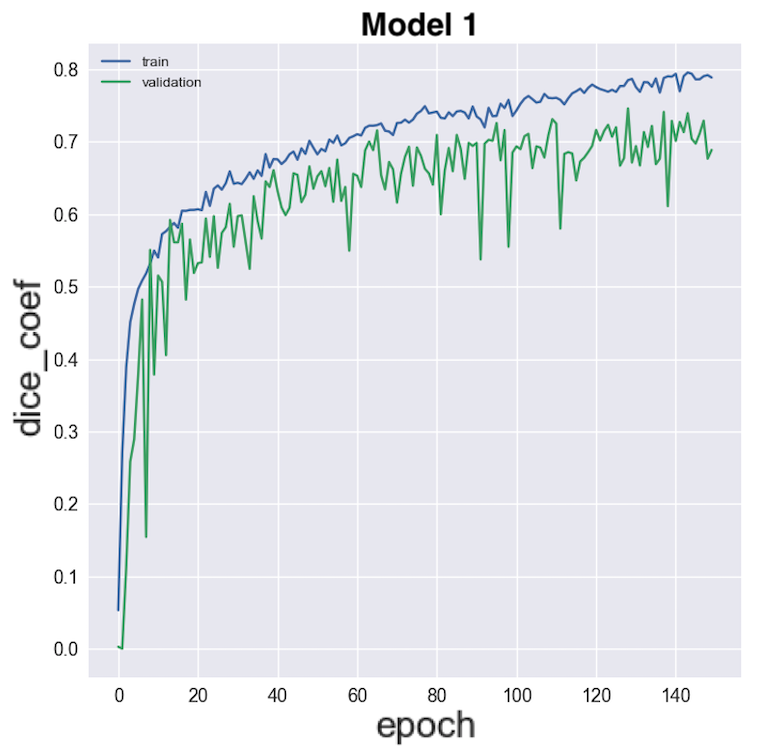
\includegraphics[width=0.49\textwidth]{../images/dice_coef1.png}
	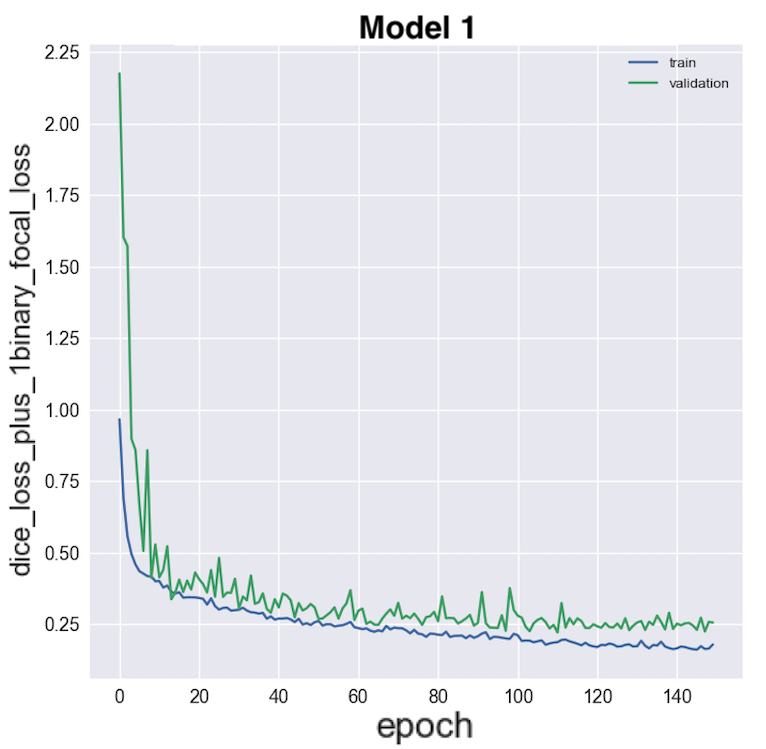
\includegraphics[width=0.49\textwidth]{../images/loss1.png} 

    \caption{Training (blue) and validation (green) model history plots for Model 1. \textit{Left}): model dice coefficient as a function of the epochs. \textit{Right}): model loss as a function of the epochs.}
    \label{training1}
    
\end{figure}


\begin{figure}[htp]

    \centering
    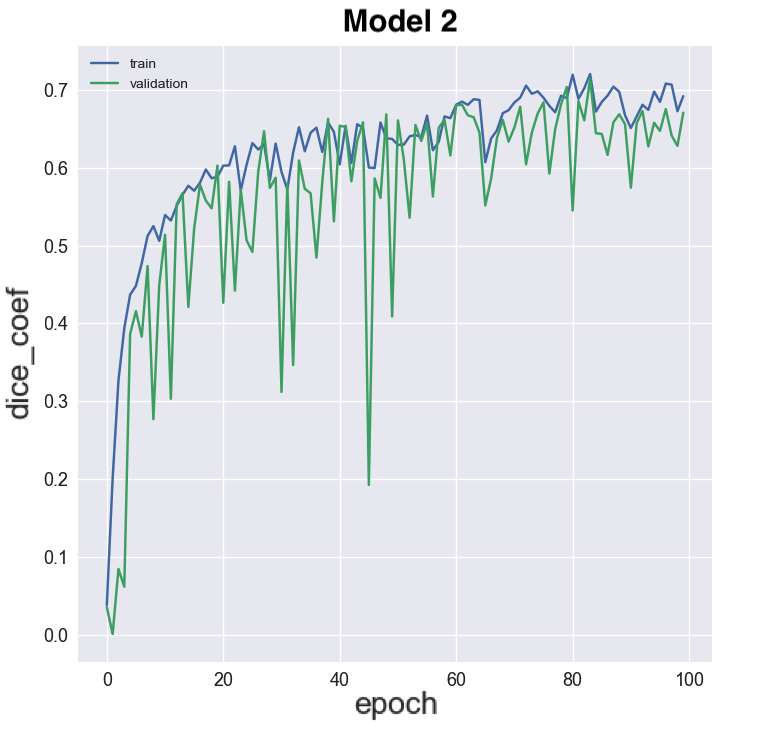
\includegraphics[width=0.49\textwidth]{../images/dice_coef2.png}
	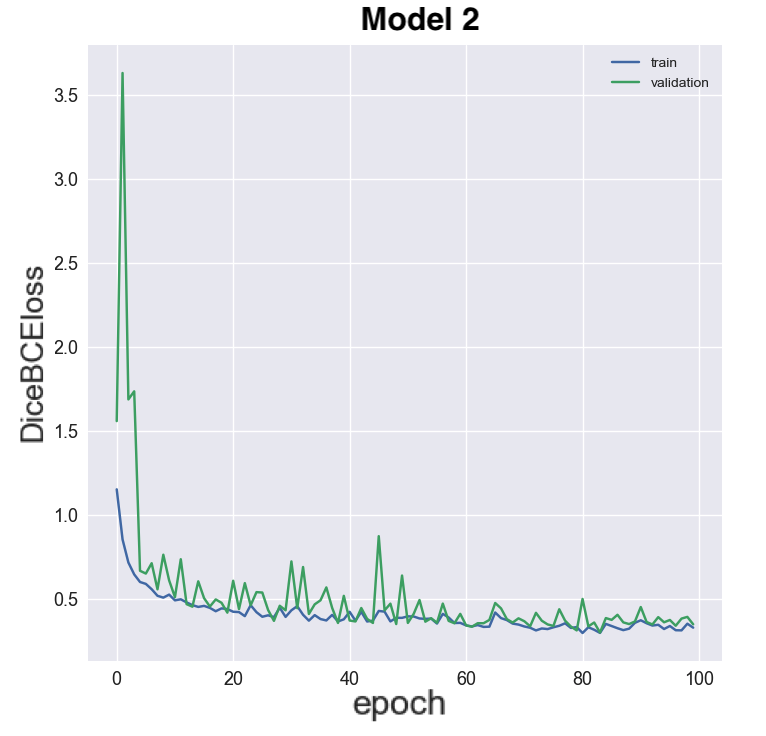
\includegraphics[width=0.49\textwidth]{../images/loss2.png}

    \caption{Training (blue) and validation (green) model history plots for Model 2. \textit{Left}): model dice coefficient as a function of the epochs. \textit{Right}): model loss as a function of the epochs.}
    \label{training2}
    
\end{figure}


\newpage

\begin{figure}[htp]

    \centering
    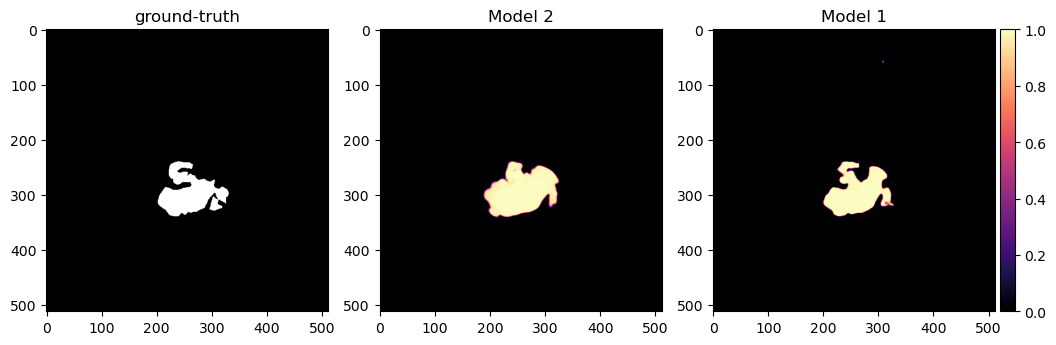
\includegraphics[width=\textwidth]{../images/predcomparison.png}
    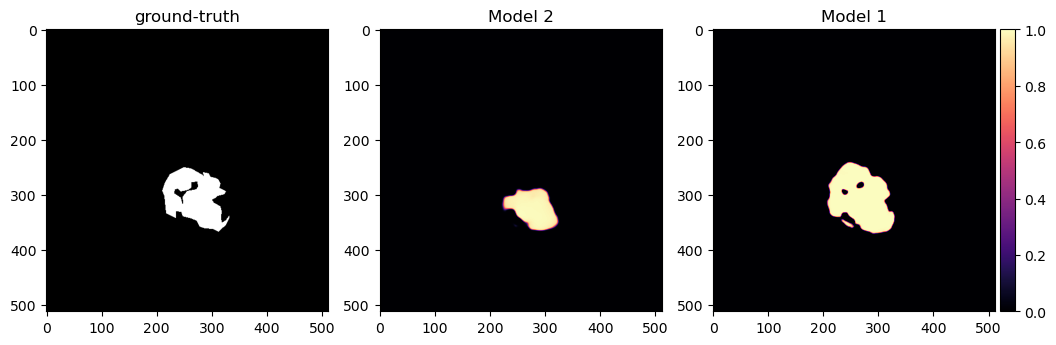
\includegraphics[width=\textwidth]{../images/predcomparison1.png}
    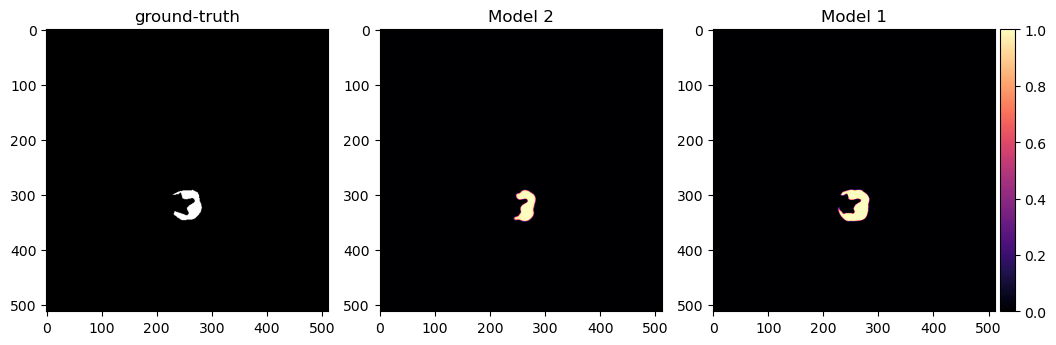
\includegraphics[width=\textwidth]{../images/predcomparison2.png}
    

    \caption{Comparison between the ground-truth image and the prediction of both models. 
    The first column represents the input image. 
    The second one represents the prediction of Model 2. 
    The third one represents the prediction of Model 1.
    The prediction is plotted as a probability density map between 0. and 1. as shown by the sequential colormap.}\label{predcomparison}

\end{figure}


\begin{figure}[htp]

    \centering
    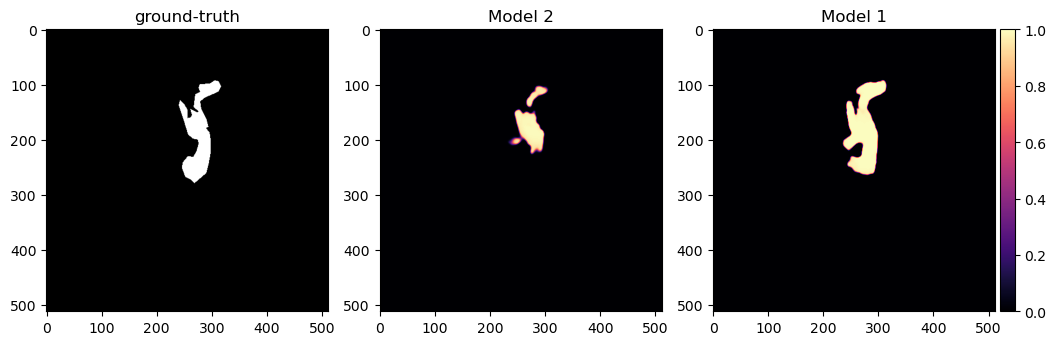
\includegraphics[width=\textwidth]{../images/predcomparison3.png}
    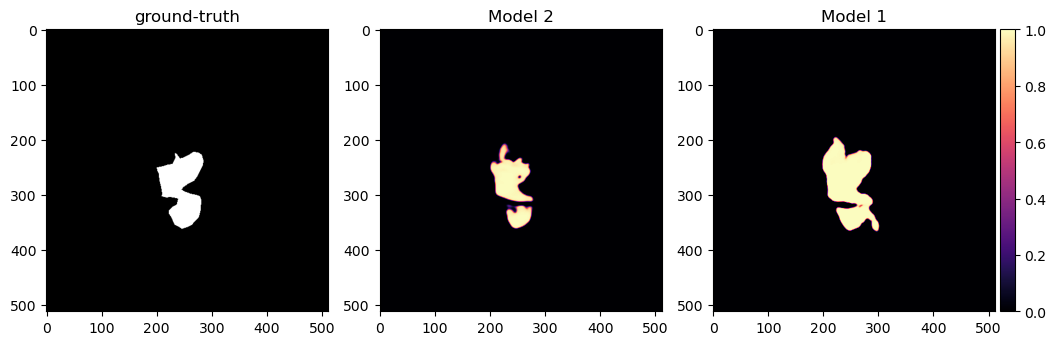
\includegraphics[width=\textwidth]{../images/predcomparison4.png}
    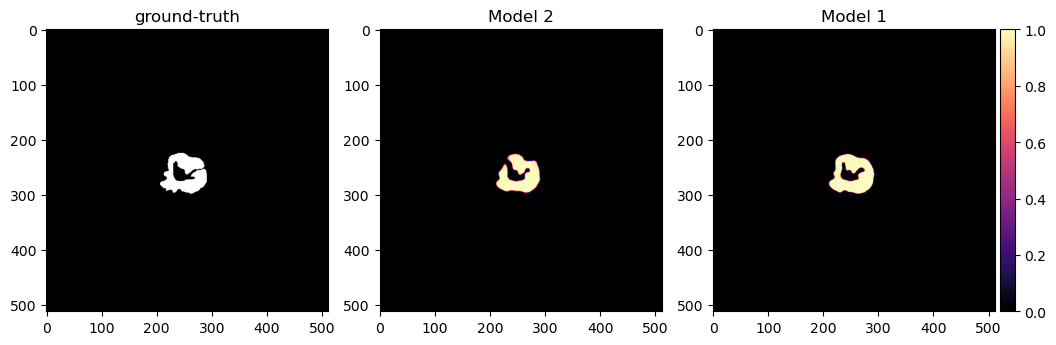
\includegraphics[width=\textwidth]{../images/predcomparison5.png}
    

    \caption{Comparison between the ground-truth image and the prediction of both models. 
    The first column represents the ground-truth image. 
    The second one represents the prediction of Model 2. 
    The third one represents the prediction of Model 1.
    The prediction is plotted as a probability density map between 0. and 1. as shown by the sequential colormap.}\label{predcomparison2}

\end{figure}

\begin{figure}[htp]

    \centering
    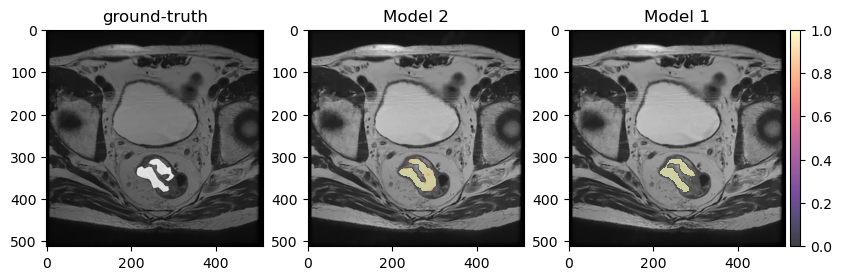
\includegraphics[width=\textwidth]{../images/predcomparisonoverlap.png}
    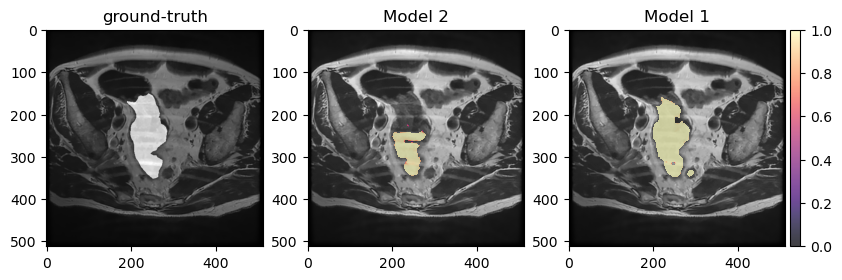
\includegraphics[width=\textwidth]{../images/predcomparisonoverlap1.png}
    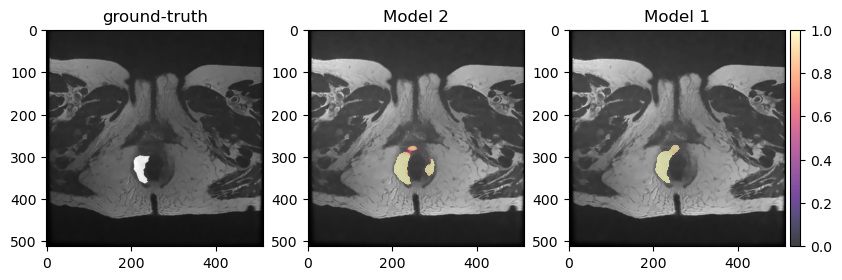
\includegraphics[width=\textwidth]{../images/predcomparisonoverlap2.png}
    

    \caption{Comparison between the ground-truth image and the prediction of both models over the input image. 
    The first column represents the ground-truth image. 
    The second one represents the prediction of Model 2. 
    The third one represents the prediction of Model 1.
    The prediction is plotted as a probability density map between 0. and 1. as shown by the sequential colormap.}\label{predcomparisonoverlap}

\end{figure}

\begin{figure}[htp]

    \centering
    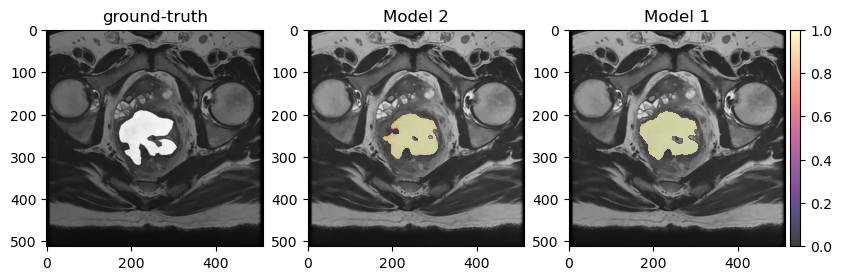
\includegraphics[width=\textwidth]{../images/predcomparisonoverlap3.png}
    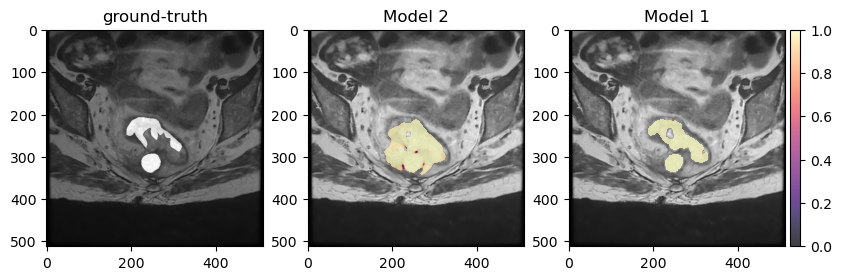
\includegraphics[width=\textwidth]{../images/predcomparisonoverlap4.png}
    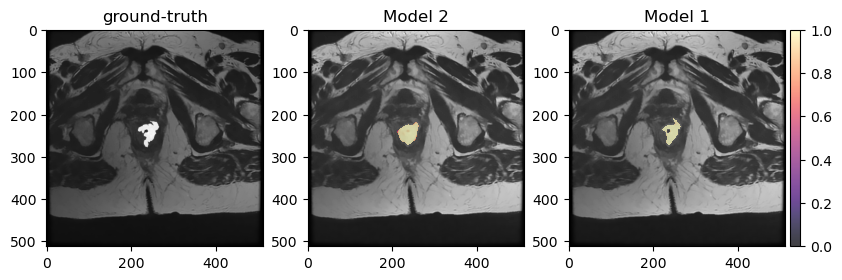
\includegraphics[width=\textwidth]{../images/predcomparisonoverlap5.png}
    

    \caption{Comparison between the ground-truth image and the prediction of both models over the input image. 
    The first column represents the ground-truth image. 
    The second one represents the prediction of Model 2. 
    The third one represents the prediction of Model 1.
    The prediction is plotted as a probability density map between 0. and 1. as shown by the sequential colormap.}\label{predcomparisonoverlap2}

\end{figure}

\end{document}